\documentclass[]{scrartcl}
\usepackage{Preamble}
\usepackage{tikz}
\usepackage{pstricks}

\setcounter{section}{7}
\newcommand{\exercise}{Exercise \thesection}
\newcommand{\duedate}{2021-01-25, 23:59}

\begin{document}
\section*{\exercise}

\subsection{Reading}
\subsection{n-Body Problem --- Partitioning/Communication Design}
\subsubsection{Memory Layout}

\begin{minted}{c++}
  std::random_device rd;  //Will be used to obtain a seed for the random number engine
  std::mt19937 gen(rd()); //Standard mersenne_twister_engine seeded with rd()
  std::uniform_real_distribution<> mass_distrib(1e-10, 1e10);
  std::uniform_real_distribution<> space_distrib(-1e3, 1e3); // start within 12km of eachother
  std::uniform_real_distribution<> vel_distrib(-1e6, 1e6); // max 0.6% speed of light

  struct Body {
    union {
      double raw[8];
      struct __attribute__((__packed__)) {
        double id;
        double m;
        double pos[3];
        double vel[3];
      };
    };
    static double uidcounter = 0;

    Body() {
      id = uidcounter;
      uidcounter += 1;

      m = mass_distrib(gen);
      for (int i=0; i < 3; i++) {
        pos[i] = space_distrib(gen);
        vel[i] = 0;
      }
    }
  }

  std::vector<Body> b(); //has to happen on one rank only for correct and unique ids
  b.resize(num_of_bodies);


  // to send we just use the raw data
  MPI_Send(&b, 8, ...)
\end{minted}

\subsubsection{Partitioning}

\begin{itemize}
  \item the amount of bodies should be a multiple of the available ranks, resulting in equally large messages
  \item each rank will handle a number of bodies
  \item the initial positions and velocities are scattered over the ranks
  \item ranks are sequential over nodes (per-slot-mapping) resulting in the least amount of node-to node communication due to circular messaging ($\frac{4}{16}$ of all communication for 16 ranks over 4 nodes)
\end{itemize}

\subsubsection{Communication}
\begin{itemize}
  \item the communication will happen in  a circular fashion
\end{itemize}

\begin{figure}[H]
  \centering
  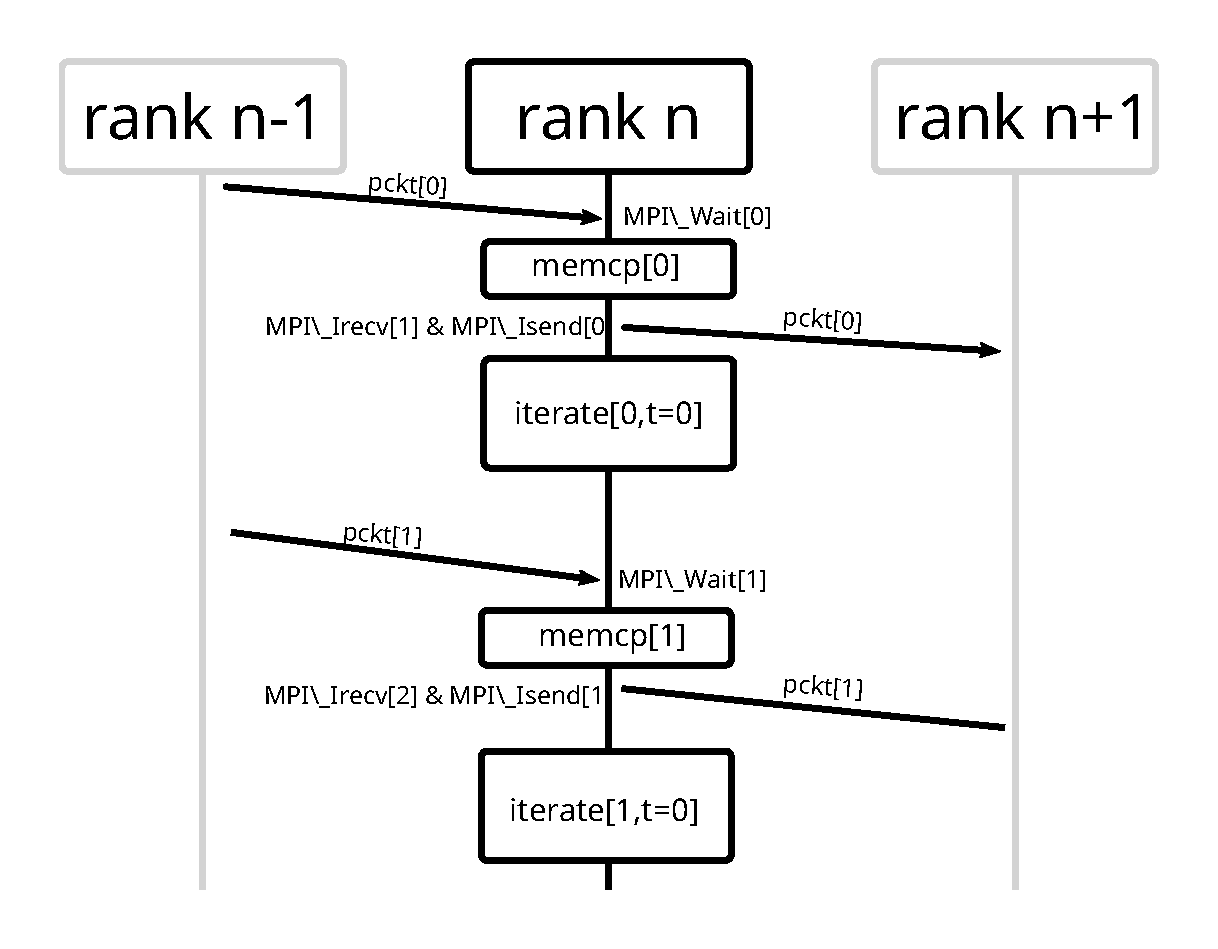
\includegraphics[width=.8\columnwidth]{./img/comm_overlap.pdf}
  \caption{}
  \label{}
\end{figure}
\end{document}
